\documentclass[a4paper]{scrartcl}

\let\chapter\section 
\let\section\subsection 
\let\subsection\subsubsection 
\let\subsubsection\paragraph 
\let\paragraph\subparagraph 
\let\subparagraph\undefined 

\usepackage{booktabs}
\usepackage[usenames,dvipsnames]{color}
\usepackage[latin1]{inputenc}
\usepackage{listings}
\usepackage[english]{babel}
\usepackage[pdftex,plainpages=false,pdfpagelabels,
    hyperfootnotes=false]{hyperref}
\hypersetup{pdftitle={GoGo -- A Go compiler written in Go},
    pdfauthor={Michael Lippautz, Andreas Unterweger},
    pdfsubject={GoGo},pdfkeywords={Go,Compiler,GoGo}}
\usepackage{graphicx}

\definecolor{lightgray}{RGB}{250,250,250}

\lstset{
    basicstyle=\small,
    frame=lines,
    backgroundcolor=\color{lightgray}
}

\title{GoGo\\ \large{A Go compiler written in Go}}
\author{
  Michael~Lippautz \\ \normalsize{\texttt{michael.lippautz@sbg.ac.at}} 
    \and 
  Andreas~Unterweger \\ \normalsize{\texttt{andreas.unterweger@sbg.ac.at}} 
}

\date{\today}

\begin{document}
  \maketitle
  \tableofcontents

  \chapter{Introduction}
    GoGo is a self-compiling (see section \ref{chpt:building}) Go compiler 
    written in Go which implements scanning, parsing and code generation for a 
    subset of the Go language \cite{goo10}. It is mostly compatible with the Go 
    compiler available at \cite{goo10} and outputs valid Plan9 assembly code 
    which can be assembled by the latter as well as the Plan9 assembly tools 
    \texttt{6a} and \texttt{6l}\cite{pik00}.\\


  \chapter{Input Language}
    Go is a programming language developed by Google, based on a C like syntax and fully specified in \cite{goo10}. The input language follows the one defined by Go. This results in programs being able to be compiled by the official Go compilers and GoGo.

    \section{Some differences to Go}
      \begin{enumerate}
        \item GoGo only provides only a \textbf{very} basic featureset. Expect 
          every advanced and interesting feature to be missing.
        \item GoGo forces the usage of semicolons at the end of statements, 
          while in actual Go this token is optional. This restriction was made 
          to make parsing easier.
        \item Go is fully Unicode compatible, while GoGo uses ASCII characters only.
        \item Simplified expressions, following Wirth's defintions\cite{wir96}.
      \end{enumerate}

    \section{EBNF}
    \label{sec:ebnf}
      The following section deals with the input language specification in 
      EBNF form. Additionally to the specification below, GoGo also allows 
      source code comments following the C++ multiline style(\texttt{/* ... */}) 
      and the C inline style (\texttt{//}).

      \subsection*{Atoms}
        The following listing describes the basic atoms that are possible in 
        GoGo programs.
        \begin{lstlisting}[caption=Atoms]
single_char = CHR(32)|...|CHR(127).
char = "'" single_char "'".
string = """ {single_char} """.

digit = "0"|...|"9".	
integer = digit {digit}.

letter = "a"|...|"z"|"A"|...|"Z"|"_".
identifier = letter { letter | digit }.
selector = { "." identifier 
    | "[" (integer | identifier selector) "]" }.
        \end{lstlisting}

      \subsection*{Expressions}
        Although not as expressive as the ones from Go, these rules define expressions that have comparisons, relations and arithmetical terms. 

        \begin{lstlisting}[caption=Expressions]
cmp_op = ">" | "<" | ">=" | "<=" | "==" | "!=".
unary_arith_op = "+" | "-".
binary_arith_op = "*" | "/" .

factor = identifier selector | integer | char | string 
    | "(" expression ")" | "!" factor.	
term = factor { (binary_arith_op | "&&") factor}.
simple_expression = [ unary_arith_op ] term 
    { (unary_arith_op | "||") term }.
expression = "&" identifier selector 
    | simple_expression [ cmp_op simple_expression ].
        \end{lstlisting}

      \subsection*{Types and Variable Declarations}

        \begin{lstlisting}[caption=Types]
type = ([ "[" integer "]" ] identifier | "uint64" | "byte") 
    | "string".
var_decl = "var" identifier type [ "=" expression ] ";".
var_decl_list = { var_decl }
        \end{lstlisting}

      \subsection*{Structs}

        \begin{lstlisting}[caption=Structs]
struct_var_decl = identifier type ";".
struct_var_decl_list = { struct_var_decl }.
struct_decl = "type" identifier "struct" "{" 
    struct_var_decl_list "}" ";".
struct_decl_list = { struct_decl }. 
        \end{lstlisting}

      \subsection*{Statements}

        \begin{lstlisting}[caption=Statements]
package_stmt = "package" identifier ";".
import_stmt = "import" string.
import_stmt_list = { import_stmt }.

stmt_sequence = { stmt }
stmt = assignment ";" | function_call_stmt ";" | if_stmt 
    | for_stmt | ";".

assignment = identifier selector "=" expression
if_stmt = "if" expression "{" stmt_sequence "}" [ else_stmt ].
else_stmt = "else" "{" stmt_sequence "}".
for_stmt = "for" [assignment] ";" [expression] ";" [assignment] 
    "{" stmt_sequence "}".
        \end{lstlisting}

      \subsection*{Functions}

        \begin{lstlisting}[caption=Functions]
expression_list = expression { "," expression }.
function_call = "(" [expression_list] ")".
function_call_stmt = identifier selector function_call.

identifier_type = identifier [ "*" ] type.
identifier_type_list = [ identifier_type 
    { "," identifier_type } ].
func_decl_head = "func" identifier "(" identifier_type_list ")"  [type].
func_decl = "{" var_decl_list stmt_sequence 
    ["return" expression ";"] "}".
func_decl_raw = ";".
func_decl_list = { func_decl_head (func_decl | func_decl_raw) 
        \end{lstlisting}

      \subsection*{The GoGo Program}
        Finally, the main program structure is defined by \texttt{go\_program}. The sequence of the various program parts has been forced to the following to make parsing easier.

        \begin{lstlisting}[caption=GoGo Program]
go_program = package_stmt import_stmt_list struct_decl_list 
    var_decl_list func_decl_list.
        \end{lstlisting}


  \chapter{Output Language}
    The output language is Plan-9 assembler \cite{pik00}. It is a modified version of 64 bit assembly for Intel x86 processors with AT\&T syntax that has been created by Bell Labs to be used in their compiler and assembler collection.
    
    \section{Assembly output}
      GoGo creates an output file with assembly instructions and comments using mnemonics for op codes and operands/registers which means that it outputs in text form, not in binary form. Thereforce, an assembler is needed to process the output in order to make it executable. Like the Go compiler, GoGo relies on \texttt{6a} and \texttt{6l} of the Plan9 tools in order to acomplish this\cite{pik00}.\\
      The assembly output consists basically of three sections: the data segment, the initialization segment and the code segment. GoGo's assembly output framework provides basic output routines which make it possible to switch between those three segments. Whereas the data segment is used to reserve space for global variables and strings in the data segment, the initialization segment and the code segment contain the code for global variable initialization and the functions from the input, respectively. All other functions (code generation for arithmetical expressions etc.) rely on the assembly output framework which is also able to place comments with the corresponding input file name and line number for debugging purposes in the output file.

  \chapter{Scanner / Parser}
    The scanner is basically the provider of tokens that are used by the parser
    to process the code. In order to generate these tokens, the scanner reads
    the file character by character. If a sequence is known, it converts this 
    sequence of characters into the corresponding token. Tokens generated this
    way are called simple tokens, as they can be generated right away. For 
    instance, the sequence \textit{'A'} can be directly converted into a token 
    representing the byte value 65. \\
    Before providing a token to the parser, the scanner may convert such 
    simple tokens one more time. These complex tokens are generated from simple
    ones that represent \texttt{identifiers}. \texttt{Identifiers} are compared to a 
    predefined list of keywords. If a keyword matches a token value, the token
    is converted to the one representing the keyword. Table \ref{tbl:tokens} 
    lists some of these tokens.

    \begin{table}[htb]
    \centering
    \begin{tabular}{ll}
        \toprule
        Simple tokens & \texttt{\&\&}, \texttt{+}, \texttt{-}, \texttt{\{}, \texttt{\}}, \texttt{$($}, \texttt{$)$}, \dots \\
        Complex tokens & \texttt{for}, \texttt{if}, \texttt{else}, \texttt{func}, \texttt{type} \\
        \bottomrule
    \end{tabular}
    \caption{Token examples}
    \label{tbl:tokens}
    \end{table}

    The scanner also implements a very simple escaping mechanism that allows 
    sequences like \textit{'\textbackslash n'} to be used in strings. \\
    Comments can be written as \textit{/* ... */} blocks or 
    \textit{\textbackslash \textbackslash} until the line ending, like in C/C++.
    \\ \\
    The parser then takes these tokens and represents the language defined by
    the EBNF from section \ref{sec:ebnf}. The parser is basically implemented 
    as LL1 like in \cite{wir96}, with one minor difference. In order to be 
    compatible with Go it was necesarry to include one namespace hierachy that 
    is represented by packages. Since this name scope is prefixed 
    using \texttt{package.}, the parser needs a lookup of three (LL3)in this 
    case.

  \chapter{Symbol table}
    In order to be able to lookup local and global variable names as well as function names, a symbol table is required. Based on \cite{wir96}, object and type descriptors were used, each containing the information required for lookup and code generation. Object descriptors are used to store information about variables and parameters whereas type descriptors are used to store information about types and functions.\\
    The following tables \ref{tbl:objectdesc} and \ref{tbl:typedesc} summarize the fields of the object and type descriptors and their respective purpose. Some fields had to be added in order to support forward declarations and the distinction between values and pointers.
      \begin{table}[htb]
      \centering
      \begin{tabular}{lcl}
        \toprule
        \textbf{Field} & \textbf{Type} & \textbf{Purpose}\\ 
        \midrule
        Name & \texttt{string} & The object's name\\
        PackageName & \texttt{string} & The object's package (Go name space)\\
        Class & \texttt{uint64} & The descriptors's kind (variable, field, parameter)\\
        ObjType & \texttt{*TypeDesc} & The object's type\\
        PtrType & \texttt{uint64} & If 1, the object's type is \texttt{*ObjType}; if 0, \texttt{ObjType}\\
        Next & \texttt{*ObjType} & Next object (linked list)\\
        \bottomrule
      \end{tabular}
      \caption{ObjectDesc}
      \label{tbl:objectdesc}
      \end{table}

      \begin{table}[htb]
      \centering
      \begin{tabular}{lc p{0.6\textwidth}}
        \toprule
        \textbf{Field} & \textbf{Type} & \textbf{Purpose}\\
        \midrule
        Name & \texttt{string} & The type's/function's name\\
        PackageName & \texttt{string} & The type's/function's package (Go name space)\\
        ForwardDecl & \texttt{uint64} & If 1, the type/function has not yet been fully delcared/implemented\\
        Form & \texttt{uint64} & The descriptor's kind (simple type, array type, struct type, function)\\
        Len & \texttt{uint64} & For simple types: type size in bytes, for arrays: array size\\
        Fields & \texttt{*ObjDesc} & For struct types: struct fields, for functions: function parameters\\
        Base & \texttt{*TypeDesc} & For array types: the array base type\\
        Next & \texttt{*TypeDesc} & Next type/function (linked list)\\
        \bottomrule
      \end{tabular}
      \caption{TypeDesc}
      \label{tbl:typedesc}
      \end{table}

    For both global and function-local symbol tables the build-up and lookup is integrated into the parser. Whenever sufficient information (variable name, function name, type name; optionally preceeded by a package name) is encountered, a lookup in the symbol table is issued. Declarations issue new symbol table entries with the corresponding descriptor properties as described above.\\
    Forward declarations are currently only supported for type pointers (as pointers are always 64 bits in size) and functions (as the affected offsets can be fixed by the linker if necessary). Whenever supported forward declarations are encountered, a new symbol table entry is created with \texttt{ForwardDecl} set to 1. Forward declared function can then be called, although forward declared type pointers cannot be dereferred until the size of the type they are pointing to is known (\texttt{ForwardDecl} is 0). When forward declared functions are implemented, the corresponding symbol table entry is modified (\texttt{ForwardDecl} is set to 0) instead of creating a new one.
      
    \section{Supported data types}
      GoGo supports 4 built-in value types and the declaration of new struct and array types as well as pointers to value, struct and array types. The 4 built-in data types are based on the data types supported by the Go compiler and form a minimal subset of them in order to perform basic integer and string operations. The following table \ref{tbl:types} lists the built-in value types, together with their purpose and size.
      
      \begin{table}[htb]
      \centering
      \begin{tabular}{cc p{0.5\textwidth}}
        \toprule
        \textbf{Type} & \textbf{Size} & \textbf{Purpose}\\
        \midrule
        \texttt{uint64} & 8 bytes (64 bits) & Unsigned integer with the target platform's register size\\
        \texttt{byte} & 1 byte (8 bits) & Single ASCII character or unsigned 8 bit integer value\\
        \texttt{string} & 16 bytes (see section \ref{String constants}) & Character sequences\\
        \texttt{bool} & 8 bytes (64 bits) & Internal type used for comparisions and jumps\\
        \bottomrule
      \end{tabular}
      \caption{Built-in types}
      \label{tbl:types}
	  \end{table}

    \section{Local variables and offset calculations}
      In order to be able to distinguish between parameters, local and global variables, a global and a local symbol table as well the function's parameters as third, virtual symbol table are used. Local variables hide global variables of the same name by performing the symbol table lookup for local variables and parameters first and returning the first match if there is any.\\
      The memory layout for local and global variables as well as parameters is equal: the object's offset address contains the first 64 bits of the object, the next highest address (offset address plus 64 bits) contains the next 64 bits etc. All local and global variable offset addresses are 64 bit aligned. The offset of an object can be calculated by summing the aligned sizes of its predecessors in the corresponding variable list. Doing this, it has to be taken into consideration that pointers always occupy 8 bytes (64 bits), regardless of the type they are actually pointing to.\\
      Global variables start at offset 0 of the data segment, referred to as \texttt{data+0} in the output. Subsequent global variables use ascending offsets as described above (p.e. referred to as \texttt{data+8} for offset 8). Local variables and parameters are addressed relative to the stack pointer \texttt{SP}, starting at offset \texttt{SP+8} for parameters with ascending offsets as described for global variables (\texttt{SP} is reserved for the saved instruction pointer \texttt{IP}, see \ref{The generation of functions}). Local variables start at offset \texttt{SP-8} in descending order (\texttt{SP-16} for the second 64 bit variable, \texttt{SP-24} for the third etc., see table below) in descending order. Ignoring the sign, the offset relative to SP is still in ascending order, so the offset calculation method as used for global variables and parameters can be used.\\ \\
      \begin{table}[h]
      \begin{tabular}{llp{2cm}l}
        \cmidrule{1-2}
        \textbf{Address} & \textbf{Content} & & \textbf{Source code}\\
        \cmidrule{1-2}
        \texttt{SP-0} & Saved \texttt{IP} & & \\
        \texttt{SP-8} & \texttt{a} & & \texttt{var a uint64;}\\
        \texttt{SP-16} & \texttt{b} & & \texttt{var b uint64;}\\
        \texttt{SP-24} & \texttt{c} & & \texttt{var c uint64;}\\
        \texttt{SP-32} & \texttt{s} (higher 8 bytes) & & \texttt{var s string;}\\
        \texttt{SP-40} & \texttt{s} (lower 8 bytes) & & \\
        \cmidrule{1-2}
      \end{tabular}
      \end{table}\\ \\
      As global and local variables as well as parameters share the same offset calculation as described above, they can be treated equally with no change of the offset calculation mechanism. When printing a reference to a variable address in the output, the relative offset does not need to be changed, only the reference address (the beginning of the data segment, \texttt{data}, or \texttt{SP} respectively) and the offset's sign. This requires the variable's kind (local, global, parameter) to be stored during code generation until both address and offset are needed. This is done by introducing a new field named \texttt{Global} to the \texttt{Item} type (see next section), indicating whether an object is a global or a local variable or a parameter, respectively.\\
      Offset calculations within types (p.e. calculating the field offsets in a struct or an array index) require a slightly different handling. Global variables as well as parameters can be treated the same way as explained above as their internal offsets' ascending order corresponds to their memory layout (ascending addresses). Local variables require a different calculation as their memory layout (descending addresses) differs. This is necessary in order to be able to assign global to local variables and vice verse so that their internal memory layouts correspond from the programmer's point of view. This is also done by a distinction based on the item's \texttt{Global} flag as explained above: during code generation, the internal offset of a local variable has to be calculated by subtraction instead of addition due to the negative sign of the offset (also see table above).

  \chapter{Code generation}
    GoGo emits assembly code in text form based on the Go input files. This section briefly explains the main features implemented in the code generating functions of GoGo.

    \section{Register allocation}
        The target architecture provides 8 general purpose registers (\texttt{R8}-\texttt{R15}) as well as the registers \texttt{RAX}, \texttt{RBX}, \texttt{RCX} and \texttt{RDX}\cite{int09}. The latter are not being used by GoGo to store variables as their values may change when performing arithmetical operations (p.e. \texttt{RAX} and \texttt{RDX} are always used as the destination registers for multiplications), thus possibly overwriting values previously stored there.\\
        GoGo stores a list for every one of the 8 registers currently free, returning the first free register if required by the code generator. Whenever a register is no longer required (freed), it will be reinserted into the "free" list in order to make it available for future use. Due to the limited amout of registers, the list described is implemented in form of a bit array in the compiler.

    \section{The generation of arithmetical expressions}
      As described in \cite{wir96}, code generation for arithmetical expressions basically relies on an operand stack and delayed code generation based on \texttt{Items}. For constant operands, constant folding is applied; variable operands are loaded into a free register in order to perform arithmetical operations on them.\\
      GoGo makes use of the capabilities of the target architecture by not loading constants into registers, thus reducing the number of registers required. Consider the expression \texttt{a + b} where both \texttt{a} and \texttt{b} are variables of type \texttt{uint64} with negative offsets 8 and 16 relative to the stack pointer. As the target architecture is able to perform an operation like \texttt{ADDQ R8, -16(SP)} (add the value at address \texttt{SP-16} to the register \texttt{R8}), only \texttt{a} needs to be loaded into a register, whereas \texttt{b} can be directly incorporated into the instruction itself.\\
      Multiplication and division on the target architecture both require special treatment: The multiplication instruction only takes the second operand and requires the first operand to be in the register \texttt{RAX}\cite{int09}. Therefore, the first operand has to be loaded into \texttt{RAX} prior multiplication. The multiplication result is stored as 128 bit value in \texttt{RDX} (upper 64 bits) and \texttt{RAX} (lower 64 bits). As GoGo does not support data types other than \texttt{byte} and \texttt{uint64}, the upper 64 bits in \texttt{RDX} are ignored, and the lower 64 bits are moved to one of the 8 registers to save the result before another multiplication is being performed. Similarly, division allows for an 128 bit operand (also in \texttt{RDX} and \texttt{RAX}). As GoGo does not support 128 bit size data types, \texttt{RDX} is always being zeroed prior division.\\
      The addition, substraction and multiplication operations are also used for offset calculations. Thus, an additional distinction per \texttt{Item} is required in order to be able to distinguish between addresses and values stored in registers. As arithmetical operations on \texttt{byte} and \texttt{uint64} types always operate on a value, the actual value to be calculated with has to be loaded prior calculation. As offset calculations always require the address to be loaded into the register instead of the value, it has to be made sure that the address is loaded, not the value. In order to distinguish between addresses and values in registers, the \texttt{A} field of the \texttt{Item} structure is used. Additionally, the code generation routines for addition and subtraction have an additional parameter specifying whether to calculate with addresses or values, issuing the necessary dereferencing operations if required.

    \section{The generation of assignments}
      As pointer types are supported, type checks in assignments as well as the assignments themselves get harder to implement as additional cases have to be dealt with. Additionally, the possible occurrence of the address operator (\texttt{\&}) on the right hand side of an assignment doubles the number of cases. The following table \ref{tbl:assigntypes} illustrates the distinctions made and the code generated for some of the cases allowed by the EBNF (* denotes pointer types, LHS and RHS are the \texttt{Items} on the left and right hand side, respectively). For the sake of clearity, only the cases with a non-pointer type variable \texttt{Item} on the left hand side and no address operator on the right hand side using \texttt{uint64} types are shown. The compiler is also able to assign \texttt{byte} values to one another as well as to \texttt{uint64} types.

      \begin{table}[htb]
      \begin{tabular}{lll}
        \toprule
        \textbf{LHS type} & \textbf{RHS type} & \textbf{Code/Error generated}\\
        \midrule
        Variable & Constant & \texttt{MOVQ \$RHS.A, (LHS.A)}\\
        Variable & Constant* & Type error\\
        Variable & Variable & \texttt{MOVQ (RHS.A), R\textit{temp} | MOVQ R\textit{temp}, (LHS.A)}\\
        Variable & Variable* & Type error\\
        Variable & Register with value & \texttt{MOVQ RHS.R, (LHS.A)}\\
        Variable & Register with value* & Type error\\
        Variable & Register with address & \texttt{MOVQ (RHS.R), RHS.R | MOVQ RHS.R, (LHS.A)}\\
        Variable & Register with address* & Type error\\
        \bottomrule
      \end{tabular}
      \caption{Assignment types}
      \label{tbl:assigntypes}
      \end{table}
      
      String assignments are handled separately as they require 16 bytes to be assigned. As one register can only hold 8 bytes, a second register needs to be allocated in order to perform the assignment. Although this may not be necessary in trivial cases where one string variable is assigned to another, strings in structures which require offset calculations force the use of a register when performing the offset calculation and therefore require a second register to dereference the value of the other 8 bytes. In order to be able to do this, the \texttt{C} field of the \texttt{Item} structure is being used as it is not needed for other purposes outside conditionals.

    \section{Generation of conditional expressions and control structures}
      In order to achieve condional jumps, GoGo (and thus Go) provides expressions 
      that allow comparisons (\texttt{==}, \texttt{!=}, \texttt{$>$}, \texttt{$<$},
      \texttt{$\ge$}, \texttt{$\le$}) and relative operators (\texttt{\&\&},
      \texttt{$||$}). The approach how code is generated differs from \cite{wir96}.
      Since our output language is text-based Plan9 assembly, there exists no way
      to create a fixup chain that could be used to fix conditional jumps after
      generating the code. As a result, GoGo creates labels that are then 
      translated into adresses by the Plan9 assembly tools. \\

      Since jumps are always generation after comparisons the code generation 
      for conditional jumps just needs two instructions. A \texttt{CMP} instruction
      for the actual comparison (this instruction is not bound to the comparison
      operator) and the conditional jump that takes the evaluates the registers
      of the comparison. The jumps that are needed can be seen in table \ref{tbl:jumps}.

      \begin{table}[htb]
        \centering
        \begin{tabular}{ll}
        \toprule
        \textbf{Comparisons} & \textbf{Positive Jump} \\
        \midrule
        Equal \texttt{==} & \texttt{JE}\\
        Not equal \texttt{!=} & \texttt{JNE}\\
        Greater than \texttt{$>$} & \texttt{JG}\\
        Less than \texttt{$<$} & \texttt{JL}\\
        Less than or equal \texttt{$\le$} & \texttt{JLE}\\
        Greater than or equal \texttt{$\ge$} & \texttt{JGE}\\
        \bottomrule
        \end{tabular}
        \caption{Conditional jumps used}
        \label{tbl:jumps}
      \end{table}

      The label generation (and thus the resulting labels) can be summarized as 
      follows:
      \begin{itemize}
        \item Each label has a suffix indicating whether it is used by an 
          \texttt{if/else} or \texttt{for} statement.
        \item Per convinience (Go forces this) programs compiled with GoGo
          are only allowed to have one statement (or control structure) per 
          line. A side-effect of this limitation is that the addition of line
          and column number of the expression into the label guarantees global
          uniqueness.
        \item Furthermore, an expression local counter, representing a \texttt{true} 
          or \texttt{false} branch is included.
        \item A simple prefix (used for debugging readability) makes a GoGo
          label complete.
      \end{itemize}

      In order to provide common programming constructs that involve pointer 
      comparisons (see listing \ref{lst:pointer}), GoGo uses lazy-evaluation.

      \begin{lstlisting}[label=lst:pointer,caption=Pointer comparison]
if object != nil && object.field ... {
      \end{lstlisting}

      Lazy-evaluation is provided over multiple levels of expressions using
      label merging to minimize the overhead. Each top level expression gets 
      its own stacks for \texttt{true} and \texttt{false} branching. Further 
      sub-expressions labels (in fact, just their local counters) are then 
      pushed and poped to/from the coresponding stacks. An example illustrating 
      this need is stated in \ref{lst:lazy}.
      \begin{lstlisting}[caption=Lazy-evaluation over multiple expression levels, label=lst:lazy]
if (done!=1) && (((a<1) && (b<2)) || ((c<3) && (d<4))) { ...
      \end{lstlisting}
      While the first \texttt{false} branch has to be generated for the term
      $(done!=1)$, further ones are needed for $(a<1)$ and $(c<3)$. Although these are
      \texttt{false} branches, they have different levels and result in different
      merging points.

    \subsection*{Conditional Jumps}
      GoGo provides one control structure that can be used for conditional jumps,
      namely \texttt{if}/\texttt{else}. While elseif and case statements could
      have provided further programming experience, the compiler itself uses only
      \texttt{if}. The \texttt{if}/\texttt{else} construct uses the condional
      expressions explained above and results in a structure as follows:
      \begin{table}[hbt]
        \centering
        \begin{tabular}{l}
          \toprule
          Code generated for expression\\
          \texttt{If} prolog including possible \texttt{else} jump\\
          \hspace{0.5cm} \texttt{True} body\\
          \texttt{Else} header\\
          \hspace{0.5cm} \texttt{False} body\\
          Epilog catching \texttt{true} body exit\\
          \bottomrule
        \end{tabular}
      \end{table}

    \subsection*{Loops}
      GoGo supports only \texttt{for} structures to construct loops, because
      Go doesn't offer any other form of loops itself. In order to provide a more 
      lightweight loop variant, one may skip parts of the \texttt{for} construct.
      The language construct is defined as follows:
      \begin{lstlisting}
for <initial-assignment> ; <expression> ; <loop-assignment> { ...
      \end{lstlisting}

      While usually one might use the initial-assignment and the loop-assignment
      to control the flow, they can be skipped. In fact, each part may be skipped
      to generate a very lightweight \texttt{while(true)} loop. The code that is
      usually (using all three clauses) generated has the structure:

      \begin{table}[hbt]
        \centering
        \begin{tabular}{l}
          \toprule
          \textbf{Code structure}\\
          \midrule
          Initial-assignment\\
          Expression label\\
          Expression evaluation\\
          (Jump to body if first iteration)\\
          Conditional jump to epilog depending on the expression\\
          Loop-assignment label\\
          \hspace{0.5cm} Loop-assignment\\
          Loop body label\\
          \hspace{0.5cm} Loop body\\
          Epilog catching exits\\
          \bottomrule
        \end{tabular}
      \end{table}
    

    \section{The generation of functions calls} \label{The generation of functions}
      Consider the following example with the current function having 3 local variables -- 2 of type \texttt{uint64} and one of type \texttt{string} -- calling the function \texttt{foo} which has the following prototype:
        \begin{lstlisting}
func foo(param1 uint64, param2 uint64, param3 string) uint64;
        \end{lstlisting}
      In order to be compatible to the Go calling convention, the stack is organized as follows before calling \texttt{foo}:
      \begin{table}[h!]
      \begin{tabular}{ll}
        \toprule
        \textbf{Address} & \textbf{Content}\\
        \midrule
        \texttt{SP-0} & Saved \texttt{IP}\\
        \texttt{SP-8} & Local variable 1 (uint64)\\
        \texttt{SP-16} & Local variable 2 (uint64)\\
        \texttt{SP-24} & Local variable 3 (string), higher 8 bytes\\
        \texttt{SP-32} & Local variable 3 (string), lower 8 bytes\\
        \midrule
        \texttt{SP-40} & Placeholder for return value of foo\\
        \texttt{SP-48} & \texttt{param3} of \texttt {foo}, higher 8 bytes\\
        \texttt{SP-56} & \texttt{param3} of \texttt {foo}, lower 8 bytes\\
        \texttt{SP-64} & \texttt{param2} of \texttt {foo}\\
        \texttt{SP-72} & \texttt{param1} of \texttt {foo}\\
        \bottomrule
      \end{tabular}
      \end{table}\\ \\
      As can be seen, the parameters are pushed in reverse order and share the address calculation algorithm of local variables (considering the offsets of the local variables), allowing to reuse the latter for this purpose. In order to move the parameters to their corresponding positions on the stack, the offsets are calculated and an assignment statement with the stack offset on the LHS (as variable \texttt{Item}) is being performed which allows to reuse the code for assignment generation, including all type checks and conversions. Optionally, currently used registers are pushed onto the stack between the local variables and the return value, yielding an offset correction to be considered when pushing the parameters.\\
      When calling \texttt{foo} in the above example, the \texttt{SP} is first decreased by 72, followed by another implicit decrease of 8 due to the \texttt{CALL} instruction which pushes the current \texttt{IP} onto the stack and decreases the \texttt{SP} automatically. The stack is then prepared for \texttt{foo} to which it appears similar as to the callee, with the old \texttt{IP} at offset \texttt{SP}, the parameters on positive offsets relative to \texttt{SP} and the local variables (if any) with negative offsets.
      \begin{table}[h!]
      \begin{tabular}{lll}
        \toprule
        \textbf{Address after call} & \textbf{Address before call} & \textbf{Content}\\
        \midrule
        \texttt{SP+40} & \texttt{SP-40} & Placeholder for return value of foo\\
        \texttt{SP+32} & \texttt{SP-48} & \texttt{param3} of \texttt {foo}, higher 8 bytes\\
        \texttt{SP+24} & \texttt{SP-56} & \texttt{param3} of \texttt {foo}, lower 8 bytes\\
        \texttt{SP+16} & \texttt{SP-64} & \texttt{param2} of \texttt {foo}\\
        \texttt{SP+8} & \texttt{SP-72} & \texttt{param1} of \texttt {foo}\\
        \texttt{SP} & -- & \texttt{IP} of callee\\
        \texttt{SP-8} & -- & Possible local variable of \texttt{foo}\\
        \bottomrule
      \end{tabular}
      \end{table}\\ \\
      As can be seen, the offsets before and after the call differ by \texttt{72+8=80} as explained above. GoGo does not use base or frame pointers, but relies only on the stack pointer to perform all offset calculations. The return value is always located "after" the other parameters and can be used as the RHS of an assignment with its known offset as explained with the parameters above. After the function call, 80 is added to the stack pointer in order to restore the previous stack "view" for the callee. Optionally saved registered are restored considering their additional offset in reverse order.\\
      Internally, a function is represented by a \texttt{TypeDesc} (compare table \ref{tbl:typedesc}) where the fields represent the functions parmaeters, including an optional return value at their end. When a function is being called without prior declaration, the parameter types have to be derived from the types of the expressions encountered. As the total number of parameters is unknown before the end function call in the input file, a marker is inserted in the output code and comments to indicate that the final offset has yet to be determined. As the offset due to local variables is known, it is included. Due to the marker which includes information about the name of the function called, the linker is able to adapt the unfinished offsets in order to correct them accordingly.\\
      When functions have been called, but not declared, and then called again, the type check included in the code generation for assignments is already effective and detects improper assignment types. However, it is necessary to extend this check as the first call can p.e. be with a parameter of type \texttt{byte} and the second call with a parameter of type \texttt{uint64}. This is allowed, as a \texttt{byte} type represents a subset of the \texttt{uint64} type, requiring a conversion for the former in order to assure that the 7 additional bytes are zero. This can be done by simply extending the type check of the assignment. This also applies to the return value (as it is treated like a parameter), although it has to be considered that calls of functions without return value assignments do not necessarily mean that the function called has no return value. Therefore, additional checks are necessary, including the check of the return value's existence and type when the actual function declaration is being made.

    \section{Global variable initialization}
        Besides the compiled functions from the input file, the code segment contains a function called main.init which performs the initialization of global variables. In contrast to local variables which can be initialized directly at point of their declaration, global variables need to be initialized before any other methods are called, thus requiring the main.init function.\\
        Global variables in general are stored in the data segment, called \texttt{data} in the output. They are addressed by their corresponding symbol table offsets relative to the beginning of the data segment. For the special treatment of string constants, please refer to the next section.

    \section{String constants} \label{String constants}
        Strings in Go are 16 bytes in size, containing an 8 byte address (pointer) to its character buffer and an 8 byte length (of which only 4 bytes are used). This makes string length calculations unnecessary and also explains why strings in Go are read-only and have to be reallocated when being changed.\\
        Whenever a string constant is found in the input code, a new byte array with the string's length is declared and initialized with the string's characters. Next, another 16 bytes are allocated which represent the actual string. Using the main.init function as described in the previous section, the string's length and the previously allocated byte array address are assigned to the according offsets of the string in the data segment. When assigning the string constant (or using it as a parameter), an item representing a data segment variable with the string's address is used, therefore eliminating the need for any further special treatment.

  \chapter{Library and run time}
    In order to be able to perform I/O operations and memory management, a library called libgogo is implemented which wraps Linux syscalls and provides an easy to use interface to the GoGo compiler. As GoGo generates assembly code for 64 bit Linux operating systems and the Go compiler allows to mix assembly and Go code, the operating system's built-in functions can be used via syscalls in order to provide the functionality described above.

    \section{I/O syscalls}
      Besides read and write operations to files (and the console), exiting the program as well as opening and closing files requires the use of syscalls. On Linux 64 bit operating systems with Intel architecture, these syscalls can be invoked by the assembly mnemonic \texttt{SYSCALL} where the register \texttt{RAX} contains the syscall number defining the syscall, and the registers \texttt{RDI}, \texttt{RSI} and \texttt{RDX} contain the first, second and third parameter respectively\cite{var08}.\\
      The following table \ref{tbl:syscalls} lists the syscalls used by libgogo, together with the value of \texttt{RAX} representing the syscall number. The latter were derived from the C constants defined in \texttt{/usr/src/linux-headers-2.6.32-22/arch/x86/include/asm/unistd\_64.h} of the current Linux kernel source\cite{var10}. The syscall function prototypes (for semantics and formal parameters) were derived from the corresponding Linux man pages (see \cite{var97} and others).

      \begin{table}[htb]
      \centering
      \begin{tabular}{ccc}
        \toprule
        \textbf{Syscall number (\texttt{RAX})} & \textbf{Syscall function} & \textbf{Purpose}\\
        \midrule
        0 & \texttt{sys\_read} & Reads from a file\\
        1 & \texttt{sys\_write} & Writes to a file\\
        2 & \texttt{sys\_open} & Opens a file\\
        3 & \texttt{sys\_close} & Closes a file\\
        12 & \texttt{sys\_brk} & See next section\\
        60 & \texttt{sys\_exit} & Exits the program\\
        \bottomrule
      \end{tabular}
      \caption{Syscalls}
      \label{tbl:syscalls}
      \end{table}

    \section{The memory manager}
      Libgogo provides a very simple memory manager using a bump pointer which can allocate, but not free memory. By using the \texttt{sys\_brk}\cite{var97} function, the memory manager expands the data segment of the running program in steps of 10 KB if necessary in order to deal with subsequent allocations.\\
      As the Go compiler used for boot strapping uses a custom memory manager in its run time environment, the libgogo memory manager and the GoGo compiler take measures to avoid conflicts with the former. First and foremost, all implicit and explicit memory allocations in the GoGo compiler rely on the libgogo memory manager in order to keep the amount of memory allocated by the Go run time constant. Additionally, the memory manager does not allocate any memory in the original data segment to not overwrite any string constants or other information stored there by the Go run time. This is achieved by directly expanding the data segment during the initialization of the libgogo memory manager which also allows to store the first address allocated, thus being able to distinguish between memory allocated by the libgogo memory manager and memory allocated by the Go run time.

    \section{String memory management}
      Based on the memory manager described above, functions to copy and append strings are implemented in libgogo. As strings in Go are read-only once they are created (or appended), subsequent appending operands require the string to be entirely copied to a new memory location first. In order to avoid this in most cases, the functions handling string appending in libgogo allocate more memory than needed for the current operation in order to be able to reuse this memory in subsequent append operations if the string appended is short enough to fit in the memory already allocated.\\
      Empirical testing showed that it is most convenient to allocate the next power of two of the string length required (p.e. 16 if 9 bytes are initially required). This reduces the number of copy operations and thus memory consumption by more than a power of 10 for very large strings and small appended string (which is common appending code output).\\
      The string manager also has to take care of strings which have been allocated by the Go run time as those strings don't have any "spare" bytes left. Thus, a reallocation of memory for these strings is necessary and cannot be avoided. Subsequent allocations (after the reallocation) can then be dealt with as described above, leading to the performance gains mentioned. The distinction between strings allocated by the Go run time and the libgogo memory manager can be performed easily by comparing the string's address with the first address available to the libgogo memory manager as described in the previous section. If the string's address is smaller, the string is not yet managed by the libgogo memory manager.
        
    \section{Program parameter determination}
      Usually, a program's parameters are accessible through \texttt{argc} and \texttt{argv}, positioned on the stack as function parameters of the main (entry) function. As the Go compiler used for bootstrapping adds run time routines which are invoked before the main function, the parameters cannot be fetched from the stack as their position cannot be determined. The Go compiler allows to access these parameters using a separate package (library) which could not be used in order to remain independent of third party libraries.\\
      The current approach to fetch parameters requires the activation of the \texttt{proc} file system in the Linux kernel which is enabled by default in most Linux distributions\cite{var06}. The \texttt{proc} file system allows (among other information) to access parameters of all processes running in the system, including the current process. The latter's parameters can be through the virtual file \texttt{/proc/self/cmdline} where \texttt{self} refers to the current process. The virtual file contains all parameters, separated by zero bytes and terminated by a sequence of two zero bytes. When parsed, this allows to access the program's parameters without having to access the stack.
	
  \chapter{Building / Self-compilation}
  \label{chpt:building}
    This section deals with the building process of GoGo and how self-compilation 
    is achieved.

    \section{Go language tools}
      Before introducing the compilation procedure it is important to know how
      the Go language tools (which are actually Plan9 tools) are organized.

      Each CPU architecture gets a number that is prefixed before a tool. In
      GoGo's case this would be \texttt{6}, indicating an AMD64 architecture.
      The tool suite is then organized into various compilers/linkers:
      \begin{itemize}
        \item \texttt{6a} - Assembler for AMD64 architecture (creating \texttt{*.6} 
          object files)
        \item \texttt{6g} - Go compiler for AMD64 architecture (creating \texttt{*.6}
          object files)
        \item \texttt{6l} - Linker creating an AMD64 ELF binary out of object files
      \end{itemize}
      Again, the file extensions of the object format indicate the CPU
      architecture used.

    \section{Boot-strapping}
      To create the initial compiler that is then used for subsequent 
      compilations, the Go language tools are used. Go uses \texttt{Makefile}s 
      for defining the appropriate compilation procedure. Basically, three steps 
      are needed to create the GoGo binary:      
      \begin{enumerate}
        \item Library compilation - The \texttt{6g} and \texttt{6a} tools are
          used to create a single object file containing the library code.
        \item Compiler compilation - Compile the compiler using \texttt{6g}.
        \item Link - Link the compiler object file and the library object file
          into an ELF binary using \texttt{6l}.
      \end{enumerate}
      At the end of this procedure, an architecture-dependent (AMD64) GoGo
     compiler has been created.

    \section{Self-compilation}
    \label{sec:sc}
      After creating a first bootstrapped version of the compiler, this one may
      be used for self-compilation. GoGo is written in the same language it 
      is able to compile to assembly level. Therefore, no further additions
      or changes have to be made to the source code.
      The procedure to achieve self-compilation until assembly level is shown
      in figure \ref{fig:sc}.

      \begin{figure}
        \centering
        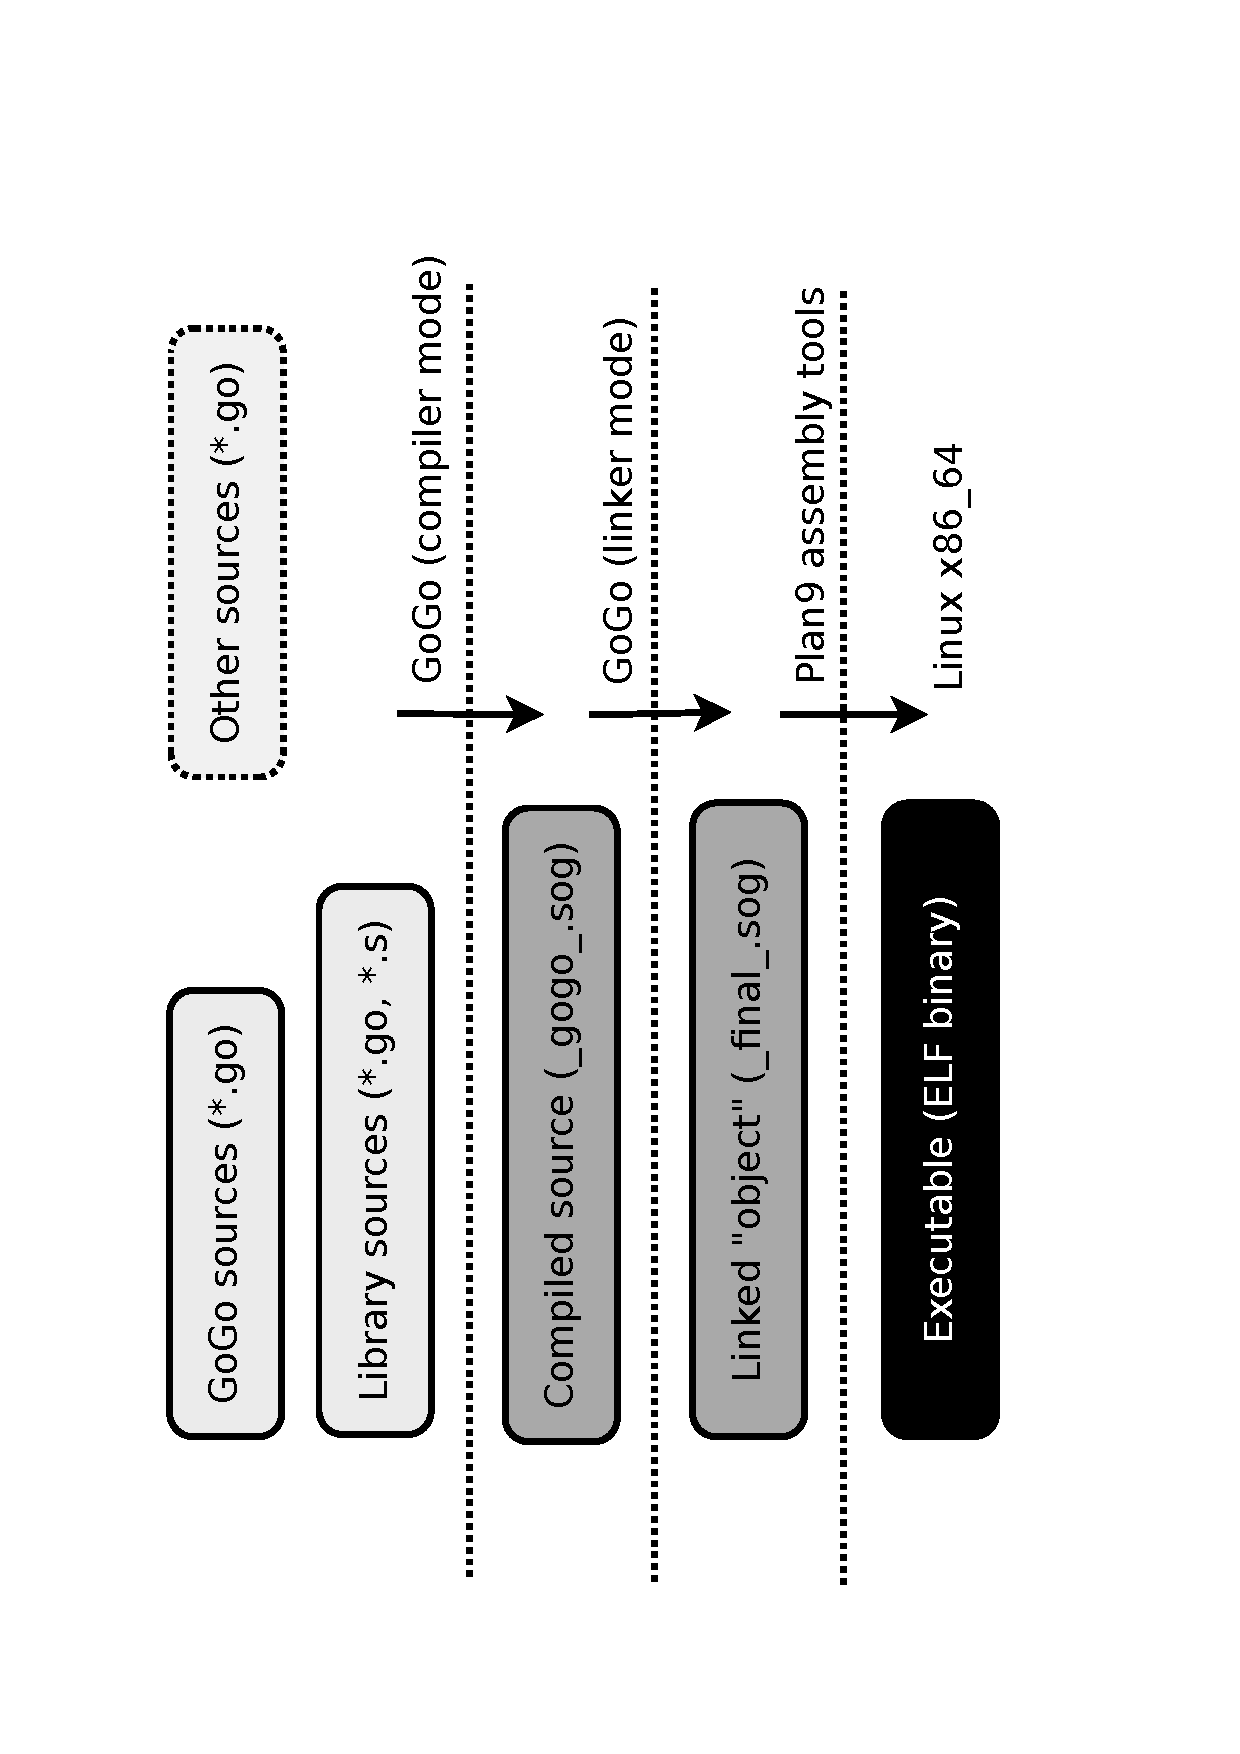
\includegraphics[scale=0.4,angle=-90,clip=true,trim=0cm 0cm 3cm 0cm]{files/building}
        \label{fig:sc}
        \caption{Self-compilation approach}
      \end{figure}  

      Although GoGo is capable of doing some very basic linking (i.e. copy 
      functions from different files and adjust the symbol table), it is not
      possible to use separate compilation during self-compilation. Altough
      function linking would work, GoGo is not able to handle global variables
      that are spread over multiple packages correctly in the linking process.
      Thus, the approach is straight-forward and can be summarized by the following:
      \begin{enumerate}
        \item All sources, this includes library, as well as compiler sources, 
          are compiled in one step. The bootstrapped compiler is used in compile
          mode for this step. 
          File ordering does not matter as long as there are no forward declared global
          variables involved (where a type has to be known). While \texttt{*.go}
          files are compiled, \texttt{*.s} files are treated as assembly and 
          directly copied into the output.
        \item The compiled source file (\_gogo\_.sog) is then again processed by
          the bootstrapped compiler in the linker mode. This mode is used to fix
          offset addresses in the parameter handling of previously forward declared functions.
        \item The received file (\_final\_.sog) then contains the compiled 
          compiler in assembly language.
        \item Finally, this file is used as input for \texttt{6a}/\texttt{6l} to
          create a platform-dependent ELF binary. This is not part of the self-compilation,
          but necessary to get an executable file.
      \end{enumerate}

      In order to perform a fixpoint-test, this procedure is used to generate 
      another instance using the previously compiled GoGo compiler. The 
      fixpoint-test passes and there are no differences in subsequent compilations.

  \chapter{Testing}
    In order to test the compiler, a test suite (using \texttt{bash}) has been 
    constructed that may be used to verify results against an already existing 
    result set. \\ \\
    The test suite offers the following functions:
    \begin{itemize}
      \item \textbf{newvalids/ackvalids/fullclean} -- These commands are used to
        create a new result set as reference for further tests. While 
        \texttt{fullclean} deletes the old set, \texttt{newvalids} is used to 
        create a new one. After verifying that the compiled output is correct 
        (by manually checking it), the command \texttt{ackvalids} can be used to 
        acknowledge the set (resulting in a checksum file). 
      \item \textbf{test/clean} -- \texttt{test} is used to perform a 
        compilation and compare the results against the last valid result set. 
        In order to do so, checksums of the tests are compared. If they are not 
        equal, a \texttt{diff} is printed to the user. \texttt{Clean} deletes
        all temporary files.
    \end{itemize}

  \bibliographystyle{alpha}
  \bibliography{gogo}

\end{document}
